\chapter{Implementierung des Triangels-to-Strip Konverters}

Die Konvertierung von Dreieckspunkten zu Strips erfolgt in der Methode \break
\lstinline{void Mesh3D::generateStrips()}. Diese Methode führt die Hauptarbeit
bei der Strip-Generierung durch, wie in den Vorlesungsfolien beschrieben
(Abbildung \ref{fig:SGI}). 

\begin{figure}[ht]
    \centering
    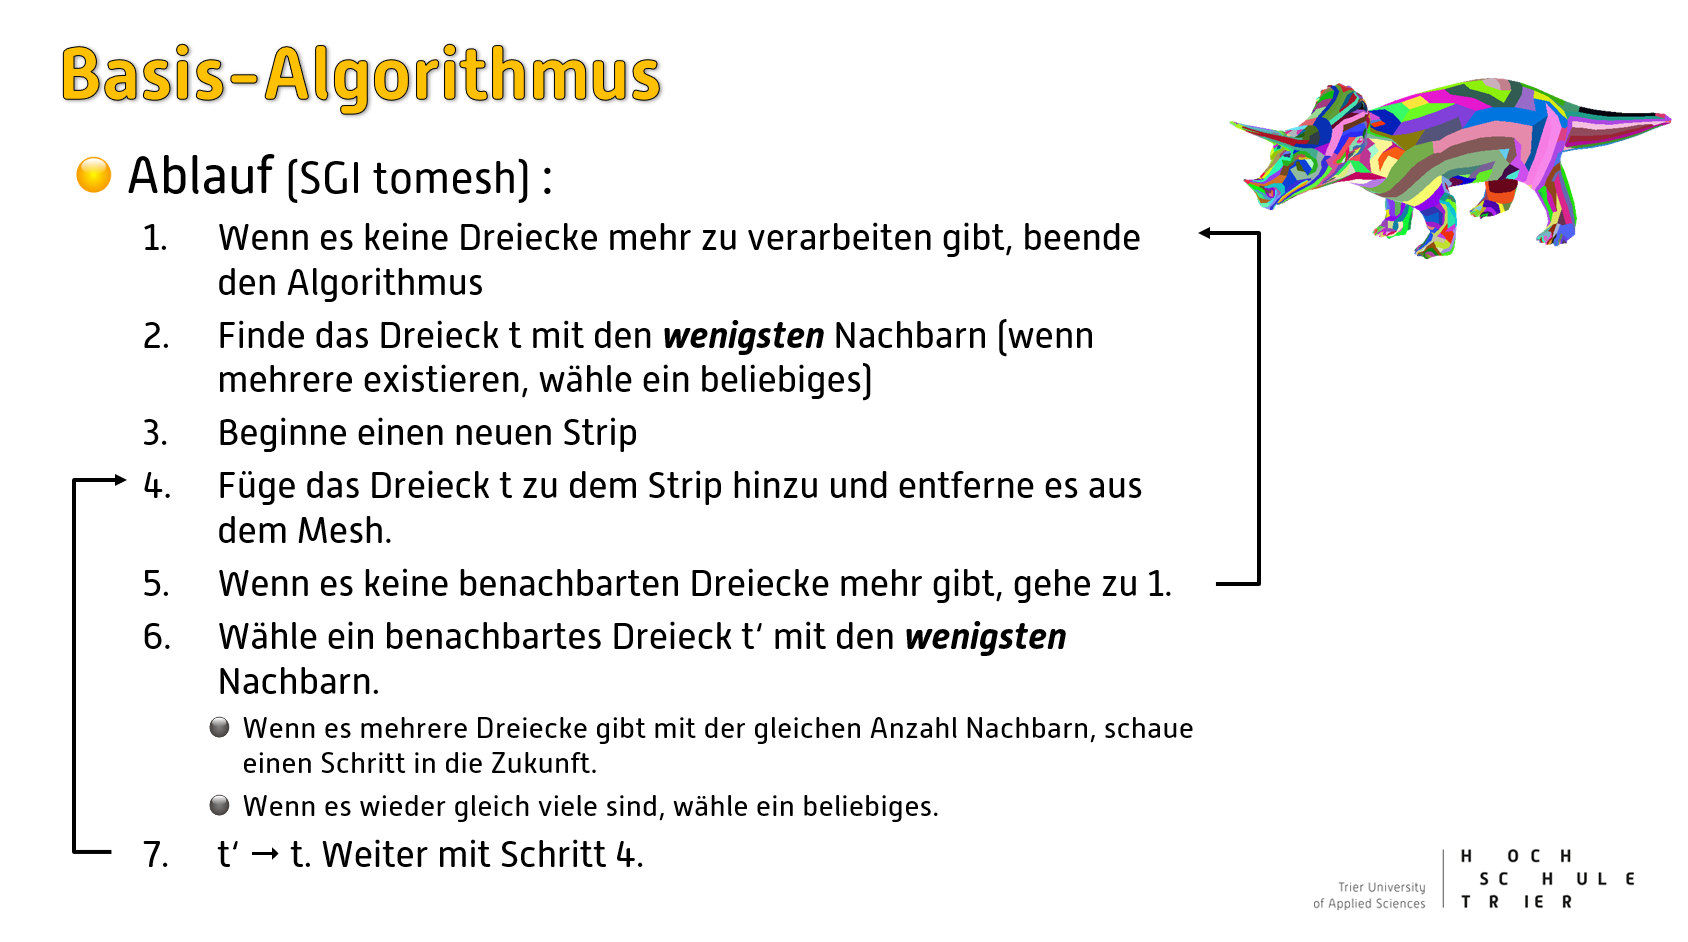
\includegraphics[scale = 0.3]{images/SGI-tomesh.PNG}
    \caption{Ablauf - SGI tomesh}
	\label{fig:SGI}
\end{figure} 
\hfil \break
Hier sind die wesentlichen Schritte und eine detaillierte Erklärung des
Algorithmus.
\begin{enumerate}
	\item \textbf{Initialisierung:} 
	\\
	Zu Beginn wird ein Vektor \lstinline{std::vector<int> triangle_indices} mit
	Indizes initialisiert, indem er inkrementell mit natürlichen Zahlen
	gefüllt wird. Diese Indizes repräsentieren die Indizes der Dreiecke im
	Vektor \lstinline{std::vector<Triangle> faces}.
	\\
	\item \textbf{Initialisierung der Nachbarn:} 
	\\
	Die Methode \lstinline{void initTriagleNeighbors()} wird aufgerufen, um das Attribut \break
	\lstinline{std::map<int, vector<int>> triangle_neighbors_indices} zu initialisieren.
	Diese Methode geht durch alle Dreiecke durch und speichert jeweils alle
	nicht-bearbeiteten Nachbardreiecke des jeweiligen Dreiecks in einen Vektor
	ab. Dieser Vektor wird an der entsprechenden Position in der Map
	gespeichert. Nicht-bearbeitete Dreiecke sind Dreiecke, die noch nicht Teil
	eines Strips sind. Ganz am Anfang gelten alle Dreiecke als nicht bearbeitet.
	\\
	\item \textbf{Hauptalgorithmus:} 
	\\
	Der Algorithmus beginnt eine äußere Schleife, die nur dann endet, wenn alle
	Dreiecke als bearbeitet markiert wurden. Dies wird überprüft, indem die
	Größe von \lstinline{std::unordered_set<int> processedTriangles} mit der Größe des
	Vektors \lstinline{triangle_indices} verglichen wird. Sollten die Größen gleich sein,
	kann geschlussfolgert werden, dass alle Dreiecke bearbeitet wurden.
	\\
	\item \textbf{Sortierung nach Nachbarn:} 
	\\
	Am Anfang jeder Iteration der äußeren Schleife werden die Indizes im Vektor
	\lstinline{triangle_indices} nach der Anzahl der nicht-bearbeiteten Nachbarn der
	jeweiligen Dreiecke in aufsteigender Reihenfolge sortiert, um
	sicherzustellen, dass in der aktuellen Iteration die Dreiecke mit den
	wenigsten Nachbarn immer vorne im Vektor stehen. Dieser Vektor wird jedes
	Mal neu sortiert, da sich die Anzahl der nicht-bearbeiteten Nachbardreiecke
	nach der Verarbeitung der Dreiecke unvorhersehbar ändert.
	\\
	\item \textbf{Beginn eines neuen Strips:} 
	\\
	Nachdem ein passendes Dreieck gefunden wurde, beginnt ein neuer Strip. Es
	wird die Variable \lstinline{std::vector<unsigned short> strip} deklariert, welche eine
	Liste der Vertices für einen Strip darstellt. Eine innere Schleife beginnt,
	die nur dann terminiert, wenn das aktive Dreieck \lstinline{active_triangle} keine
	weiteren nicht-bearbeiteten Nachbarn mehr hat. 
	\\
	\item \textbf{Hinzufügen von Dreiecken zu Strips:} 
	\\
	Direkt am Anfang der Schleife wird das Dreieck \lstinline{active_triangle} mit der
	Methode \lstinline{void addTriagleToStrip(const int targetIndex, vector<unsigned short>& strip)} 
	zum \break Strip hinzugefügt. Diese Methode schreibt die Vertices
	des übergebenen Dreiecks in den Vektor \lstinline{strip}. Falls \lstinline{strip} noch leer ist,
	werden die Vertices einfach hineingeschrieben, falls nicht, dann erfolgt
	eine Reihe von Überprüfungen:
	\\
	\begin{itemize}
	\item Es wird geprüft, ob die letzten zwei Vertices vom Strip im übergebenen
	Dreieck vorkommen. Falls ja, wird der Vertex in den Strip geschrieben,
	welcher nicht einer der beiden gemeinsamen Vertices war. 
	\\
	\item Sollte es nur einen gemeinsamen Vertex geben, kann davon ausgegangen
	werden, dass der zweite gemeinsame Vertex auf der drittletzten Stelle im
	Strip steht. In diesem Fall wird ein sogenannter Swap vorgenommen. Dabei wird das
	drittletzte Element des Strips kopiert und zwischen dem vorletzten und
	letzten Element eingefügt.
	\end{itemize} 
	
	\item \textbf{Wahl eines neuen Nachbardreiecks:} 
	\\
	Nach dem Abschluss der \lstinline{addTriagleToStrip}-Methode wird ein Nachbardreieck von
	\lstinline{active_triangle} gewählt, das die wenigsten Nachbarn hat und noch nicht
	bearbeitet wurde. Dazu wird der passende Vektor mit Nachbardreiecken aus der
	Map \lstinline{triangle_neighbors_indices} genommen und nach der Anzahl der
	nicht-bearbeiteten Nachbarn der jeweiligen Dreiecke in aufsteigender
	Reihenfolge sortiert.
	Falls es mehrere Dreiecke mit der gleichen Anzahl an Nachbarn gibt, werden die
	Nachbarn der Nachbarn (Nachbarn zweiten Grades) verglichen. Das Dreieck mit
	der kleinsten Summe der Nachbarn zweiten Grades wird zum neuen
	\lstinline{active_triangle}. 
	\\
	\item \textbf{Abschluss der Iteration:} 
	\\
	Nachdem ein kompletter Strip erstellt wurde und \lstinline{active_triangle} keine
	weiteren Nachbarn mehr hat, wird die innere Schleife verlassen. Der erzeugte
	Strip wird zum Vektor \lstinline{std::vector<vector<unsigned short>> strips}
	hinzugefügt, welcher eine Ansammlung von Strips darstellt. 
	\\
	\item \textbf{Fortsetzung der äußeren Schleife:} 
	\\
	Die äußere Schleife wird fortgesetzt, indem ein neues Dreieck mit den
	wenigsten nicht-bearbeiteten Nachbarn erneut gewählt und ein neuer Strip
	begonnen wird. Dieser Prozess wird so lange wiederholt, bis alle Dreiecke
	als bearbeitet markiert wurden. 
	\\
\end{enumerate}
